After the research of the current state of the art we proceed with RQ2, that will be addressed by means of the research conducted during the first part of the project.
To answer it %while explaining our proposed process 
we divide the development of the software to be deployed within each robot in different items.

\textbf{Software architecture.}
We developed the Co4Robots software architecture called Self-adaptive dEcentralised Robotic Architecture (SERA).
Our architecture supports a real-time decentralized robot coordination to accomplish missions with teams of robots. 
%Furthermore, it is self-adaptive, responding to external and internal events by computing new strategies to achieve the desired goals.
SERA is inspired by and extends concepts of existing proposals for robot software architectures from the literature. 
Specifically, we inspected architectures identified by a mapping study of Ahmad et al.~\cite{Ahmad201616}, which investigated software architectures for robotics systems to identify and analyze the relevant literature. % based on 56 peer-reviewed papers.
Our architecture is a three layers architecture that is strongly influenced by the well-known work of Kramer~\cite{kramer}.
Furthermore, it is component-based, %a component-based type of architecture, 
so functionalities of the system are encapsulated in modules called ``components''.
We defined SERA by first conceiving an architecture for a single robot. 
Then, we extended and refined it in order to iteratively extend and refine the architecture towards enabling communication among robots and collective adaptations. 
Thus, all the robots have an instantiation of the reference architecture but are also able to communicate and share information with the rest of the team, enabling the collective adaptation. 
For further information regarding SERA we made available a deliverable where we presented it in detail in~\url{https://goo.gl/viW76q}.


%It is important to remark that the aim of our project is to build a system that can be easily used by not technical users, so we had to define a way for them to command the missions to the robotic team.
%For this reason we added a central station that is just used during design-time in order to allocate a graphical interface to be used by a final user.

In order to create and validate SERA we went through the following steps: %steps detailed in Section~\ref{sec:validation}.
we held eight internal meetings, tested the work in three simulated scenarios, collected feedback from partners (through six emails containing questions), held three consortium meetings, wrote one deliverable and held one integration meeting where SERA was tested.
SERA was already tested during an integration meeting of the project, where the architecture demonstrated that can support the performance of a robot achieving complex missions ---i.e. collaborative transportation and autonomous driving in a dynamic environment.

%\begin{figure*}[!t]
%\begin{center}
%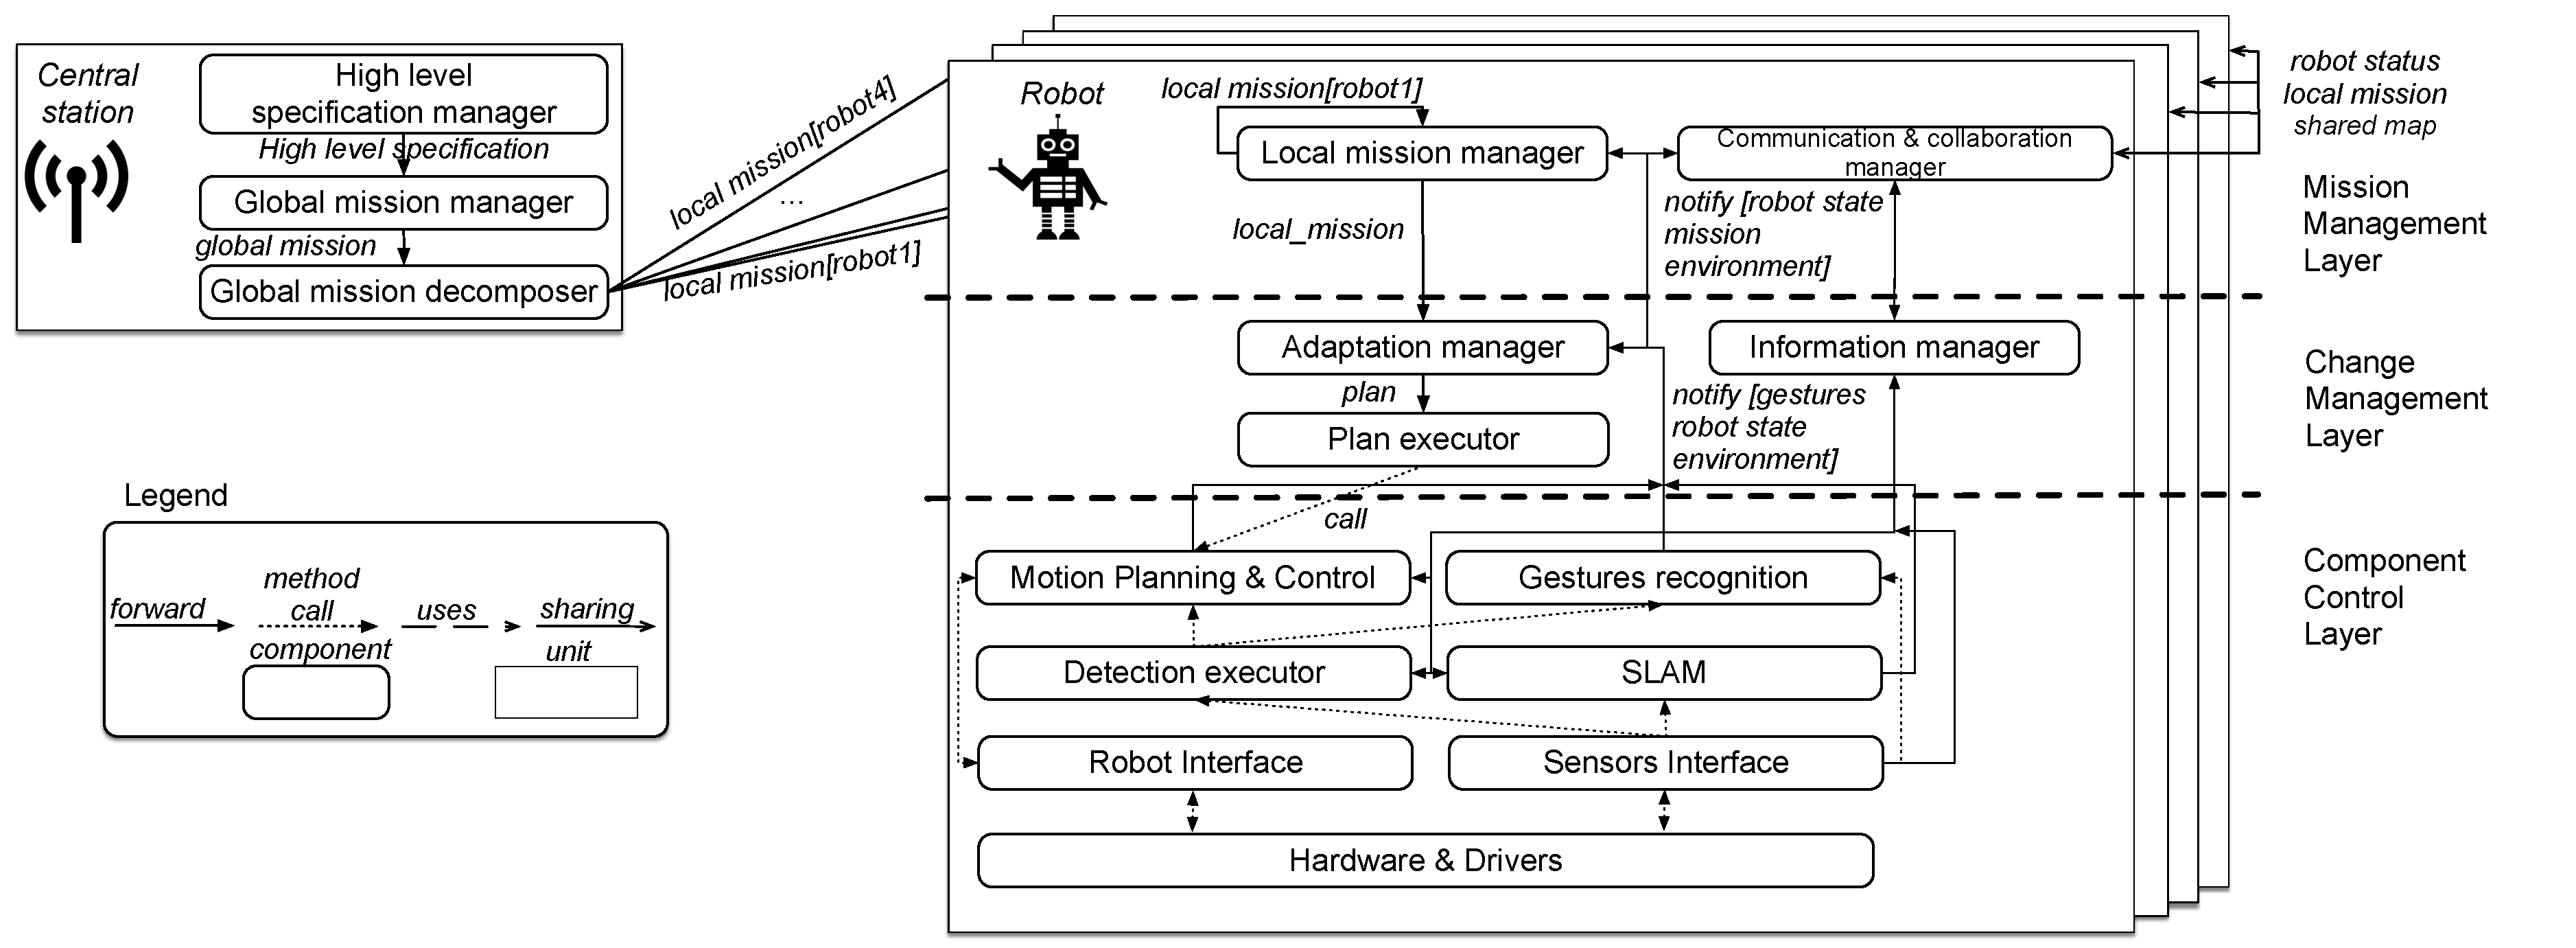
\includegraphics[width=1\linewidth]{Figures/InstanceMultiRobot_Graffle.pdf}
%\caption{Software architecture.}
%\label{fig:arch}
%\end{center}
%\end{figure*}

\textbf{Software platform.}
As explained above, the software platform will integrate the software architecture, all the generated tools and software and the configuration facilities.
The platform is also a collection of %the components that compose the architecture, a kind of library.
instantiations created by developers of each component of the architecture.
In our project, the components of our architecture are represented as ROS~\cite{Quigley2009} nodes and packages.
For this reason, the platform is based on the ROS middleware.
All these components are developed abstracting the communication problems since we rely on the interfaces defined in the architecture.
It not only significantly reduces the complexity of the code but also enforces the modularity of our system facilitating the exchange of components.
To achieve the abstraction of the interfaces, we defined an abstract class for each component where all the communication code is stored.
Then, every time a developer wants to create a new instantiation of a component he/she must create a new class  that inherits the properties of the abstract one.

%Because we not only plan to control the performance of the system that is running in each robot but also its behaviour we integrated FlexBe~\cite{Schillinger2016} in our project.
%It is a high-level behavior engine, flexibly applicable to numerous systems and scenarios.
%FlexBe not only provides a way of defining the behaviour of the robot in different scenarios (as of the study cases) by can also be used for defining the work flow.
%It also provides a graphical interface that simplifies enormously these tasks.
%FlexBe encapsulates functionalities of the robotic application, as our architecture does within components, and provides a way of orchestrate them so we keep the modularization of our system.
%As with ROS, an instantiation of FlexBe will be deployed in every robot.
%It improves the modularity, variability and reusability of our system facilitating the development of the software for animating robotic systems through the creation of reusable robot building blocks with well-defined interfaces and properties.

SERA will consider behavioural concerns to detect whether new components can be effectively plugged into the system. 
Components should be annotated with behavioural information that specifies when the component can be used (assumptions) and what the component ensures (guarantees). 
This kind of annotations can be then used to analyze whether components can be plugged into the system or whether combining specific components allows ensuring a correct system behaviour. 

Finally, in order to enable the communication between robots we implemented an approach based on ROS+REST.
So, using a suitable component that works as an interface we are able to communicate robots using services.
%In this way, each robot has an instance of ROS running in their own local environment so we can deploy a whole team of robots avoiding a central master node and the problems related with this approach (i.e. bottleneck issues, less robustness facing failures of a node, etc.), specially working with the ROS middleware.

\textbf{Configuration facilities.}
Since the components of our architecture are exchangeable our next short-term goal is to define configuration facilities that can be applied to our system. %depicted in the architecture.
Then, our robotic applications will be able to:

\begin{enumerate}
\item Being customizable at design-time, so we can configure the application components based on the requirements of our context (i.e. hardware installed in each robot, environment where they will be deployed, etc.)
\item To self-adapt or self-configure at run time, so each robot can apply changes in its configuration based on emergent events of the environment or failures of their system.
\end{enumerate}

In order to do so we will implement pluginlib\footnote{http://wiki.ros.org/pluginlib}, a package that uses ROS for writing and dynamically load plugins. %the ROS build infrastructure and provides tools for writing and dynamically load plugins.



